\chapter{Time Travelling and Fixing Bugs with Property-Based Testing - Oskar Wickström}

\begin{quotation}
\noindent\textit{\textbf{William Yao:}}
\textit{Another large-ish case study of using property-based testing, this time introducing a technique to help ensure that you’re genuinely testing enough of your code’s input space.}

\vspace{\baselineskip}
\noindent\textit{Original article: \cite{time_travelling}}
\end{quotation}


Property-based testing (PBT) is a powerful testing technique that helps
us find edge cases and bugs in our software. A challenge in applying PBT
in practice is coming up with useful properties. This tutorial is based
on a simple but realistic system under test (SUT), aiming to show some
ways you can test and find bugs in such logic using PBT. It covers
refactoring, dealing with non-determinism, testing generators
themselves, number of examples to run, and coupling between tests and
implementation. The code is written in Haskell and the testing framework
used is \href{http://hackage.haskell.org/package/hedgehog}{Hedgehog}.

This tutorial was originally written as a book chapter, and later
extracted as a standalone piece. Since I'm not expecting to finish the
PBT book any time soon, I decided to publish the chapter here.

\section{System Under Test: User Signup
Validation}
\label{system-under-test-user-signup-validation}

The business logic we'll test is the validation of a website's user
signup form. The website requires users to sign up before using the
service. When signing up, a user must pick a valid username. Users must
be between 18 and 150 years old.
Stated formally, the validation rules are:

\begin{align*} 0 < \text{length}(\text{name}) &\leq 50 \\ 18 < \text{age} &\leq 150 \end{align*} \qquad(1)

\vspace{0.8\baselineskip}


\noindent The signup and its validation is already implemented by previous
programmers. There have been user reports of strange behaviour, and
we're going to locate and fix the bugs using property tests.
Poking around the codebase, we find the data type representing the form:

\begin{minted}{haskell}
data SignupForm = SignupForm
  { formName  :: Text
  , formAge   :: Int
  } deriving (Eq, Show)
\end{minted}
And the existing validation logic, defined as \texttt{validateSignup}.
We won't dig into to the implementation yet, only its type signature:

\begin{minted}{haskell}
validateSignup
  :: SignupForm -> Validation (NonEmpty SignupError) Signup
\end{minted}
It's a pure function, taking \texttt{SignupForm} data as an argument,
and returning a \texttt{Validation} value. In case the form data is
valid, it returns a \texttt{Signup} data structure. This data type
resembles \texttt{SignupForm} in its structure, but refines the age as a
\texttt{Natural} when valid:

\begin{minted}{haskell}
data Signup = Signup
  { name  :: Text
  , age   :: Natural
  } deriving (Eq, Show)
\end{minted}
In case the form data is invalid, \texttt{validateSignup} returns a
non-empty list of \texttt{SignupError} values. \texttt{SignupError} is a
union type of the possible validation errors:

\begin{minted}{haskell}
data SignupError
  = NameTooShort Text
  | NameTooLong Text
  | InvalidAge Int
  deriving (Eq, Show)
\end{minted}



\subsection{The Validation Type}
\label{the-validation-type}

The \texttt{Validation} type comes from the
\href{https://hackage.haskell.org/package/validation}{validation}
package. It's parameterized by two types:

\begin{enumerate}
\def\labelenumi{\arabic{enumi}.}

\item
  the type of validation failures
\item
  the type of a successfully validated value
\end{enumerate}
The \texttt{Validation} type is similar to the
\href{https://hackage.haskell.org/package/base-4.12.0.0/docs/Data-Either.html\#t:Either}{Either}
type. The major difference is that it \emph{accumulates} failures,
rather than short-circuiting on the first failure. Failures are
accumulated when combining multiple \texttt{Validation} values using
\texttt{Applicative}.

Using a non-empty list for failures in the \texttt{Validation} type is
common practice. It means that if the validation fails, there's at least
one error value.

\section{Validation Property Tests}
\label{validation-property-tests}

Let's add some property tests for the form validation, and explore the
existing implementation. We begin in a new test module, and we'll need a
few imports:

\begin{minted}{haskell}
import           Data.List.NonEmpty (NonEmpty (..))
import           Data.Text          (Text)
import           Data.Validation
import           Hedgehog
import qualified Hedgehog.Gen       as Gen
import qualified Hedgehog.Range     as Range
\end{minted}
Also, we'll need to import the implementation module:

\begin{minted}{haskell}
import Validation
\end{minted}
We're now ready to define some property tests.

\subsection{A Positive Property
Test}
\label{a-positive-property-test}

The first property test we'll add is a \emph{positive} test. That is, a
test using only valid input data. This way, we know the form validation
should always be successful. We define
\texttt{prop\_valid\_signup\_form\_succeeds}:

\begin{minted}{haskell}
prop_valid_signup_form_succeeds = property $ do
  let genForm = SignupForm <$> validName <*> validAge  -- (1)
  form <- forAll genForm                               -- (2)

  case validateSignup form of                          -- (3)
    Success{}        -> pure ()
    Failure failure' -> do
      annotateShow failure'
      failure
\end{minted}
First, we define \texttt{genForm} (1), a generator producing form data
with valid names and ages. Next, we generate \texttt{form} values from
our defined generator (2). Finally, we apply the \texttt{validateSignup}
function and pattern match on the result (3):

\begin{itemize}
\item
  In case it's successful, we have the test pass with \texttt{pure\ ()}
\item
  In case it fails, we print the \texttt{failure\textquotesingle{}} and
  fail the test
\end{itemize}

The \texttt{validName} and \texttt{validAge} generators are defined as
follows:

\begin{minted}{haskell}
validName :: Gen Text
validName = Gen.text (Range.linear 1 50) Gen.alphaNum

validAge :: Gen Int
validAge = Gen.integral (Range.linear 1 150)
\end{minted}
Recall the validation rules (eq.~1). The ranges in these generators
yielding valid form data are defined precisely in terms of the
validation rules.

The character generator used for names is \texttt{alphaNum}, meaning
we'll only generate names with alphabetic letters and numbers. If you're
comfortable with regular expressions, you can think of
\texttt{genValidName} as producing values matching
\texttt{{[}a-zA-Z0-9{]}+}.
Let's run some tests:

\vspace{\baselineskip}

\begin{minipage}[l]{\textwidth}
\noindent$\lambda$\verb|> check prop_valid_signup_form_succeeds| \\
  \hspace*{1cm}\checkmark \verb|<interactive> passed 100 tests.|
\end{minipage}

\vspace{\baselineskip}

\noindent Hooray, it works.

\subsection{Negative Property Tests}
\label{negative-property-tests}

In addition to the positive test, we'll add \emph{negative} tests for
the name and age, respectively. Opposite to positive tests, our negative
tests will only use invalid input data. We can then expect the form
validation to always fail.

First, let's test invalid names.

\begin{minted}{haskell}
prop_invalid_name_fails = property $ do
  let genForm = SignupForm <$> invalidName <*> validAge -- (1)
  form <- forAll genForm

  case validateSignup form of                           -- (2)
    Failure (NameTooLong{}  :| []) -> pure ()
    Failure (NameTooShort{} :| []) -> pure ()
    other                          -> do                -- (3)
      annotateShow other
      failure
\end{minted}
Similar to our the positive property test, we define a generator
\texttt{genForm} (1). Note that we use \texttt{invalidName} instead of
\texttt{validName}.
Again, we pattern match on the result of applying
\texttt{validateSignup} (2). In this case we expect failure. Both
\texttt{NameTooLong} and \texttt{NameTooShort} are expected failures. If
we get anything else, the test fails (3).

The test for invalid age is similar, expect we use the
\texttt{invalidAge} generator, and expect only \texttt{InvalidAge}
validation failures:

\begin{minted}{haskell}
prop_invalid_age_fails = property $ do
  let genForm = SignupForm <$> validName <*> invalidAge
  form <- forAll genForm
  case validateSignup form of
    Failure (InvalidAge{} :| []) -> pure ()
    other                        -> do
      annotateShow other
      failure
\end{minted}
The \texttt{invalidName} and \texttt{invalidAge} generators are also
defined in terms of the validation rules (eq.~1), but with ranges
ensuring no overlap with valid data:

\begin{minted}{haskell}
invalidName :: Gen Text
invalidName =
  Gen.choice [mempty, Gen.text (Range.linear 51 100) Gen.alphaNum]

invalidAge :: Gen Int
invalidAge = Gen.integral (Range.linear minBound 0)
\end{minted}
Let's run our new property tests:

\begin{quote}
$\lambda$\verb|> check prop_invalid_name_fails| \\
  \hspace*{1cm}\checkmark \verb|<interactive> passed 100 tests.| \\
  \\
$\lambda$\verb|> check prop_invalid_age_fails| \\
  \hspace*{1cm}\checkmark \verb|<interactive> passed 100 tests.|
\end{quote}
All good? Maybe not. The astute reader might have noticed a problem with
one of our generators. We'll get back to that later.

\subsection{Accumulating All
Failures}
\label{accumulating-all-failures}

When validating the form data, we want \emph{all} failures returned to
the user posting the form, rather than returning only one at a time. The
\texttt{Validation} type accumulates failures when combined with
\texttt{Applicative}, which is exactly what we want. Yet, while the hard
work is handled by \texttt{Validation}, we still need to test that we're
correctly combining validations in \texttt{validateSignup}.

We define a property test generating form data, where all fields are
invalid (1). It expects the form validation to fail, returning two
failures (2).

\begin{minted}{haskell}
prop_two_failures_are_returned = property $ do
  let genForm = SignupForm <$> invalidName <*> invalidAge -- (1)
  form <- forAll genForm
  case validateSignup form of
    Failure failures | length failures == 2 -> pure ()    -- (2)
    other -> do
      annotateShow other
      failure
\end{minted}
This property is weak. It states nothing about \emph{which} failures
should be returned. We could assert that the validation failures are
equal to some expected list. But how do we know if the name is too long
or too short? I'm sure you'd be less thrilled if we replicated all of
the validation logic in this test.

Let's define a slightly stronger property. We pattern match, extract the
two failures (1), and check that they're not equal (2).

\begin{minted}{haskell}
prop_two_different_failures_are_returned = property $ do
  let genForm = SignupForm <$> invalidName <*> invalidAge
  form <- forAll genForm
  case validateSignup form of
    Failure (failure1 :| [failure2]) ->              -- (1)
      failure1 /== failure2                          -- (2)
    other                            -> do
      annotateShow other
      failure
\end{minted}
We're still not being specific about which failures should be returned.
But unlike \texttt{prop\_two\_failures\_\-are\_\-returned}, this property at
least makes sure there are no duplicate failures.

\section{The Value of a Property}
\label{the-value-of-a-property}

Is there a faulty behaviour that would slip past
\texttt{prop\_two\_different\_failures\_are\_returned}? Sure. The
implementation could have a typo or copy-paste error, and always return
\texttt{NameTooLong} failures, even if the name is too short. Does this
mean our property is bad? Broken? Useless? 
In itself, this property doesn't give us strong confidence in the
correctness of \texttt{validateSignup}. In conjuction with our other
properties, however, it provides value. Together they make up a stronger
test suite.

Let's look at it in another way. What are the \emph{benefits} of weaker
properties over stronger ones? In general, weak properties are
beneficial in that they are:

\begin{enumerate}
\item
  easier to define
\item
  likely to catch simple mistakes early
\item
  less coupled to the SUT
\end{enumerate}
A small investment in a set of weak property tests might catch a lot of
mistakes. While they won't precisely specify your system and catch the
trickiest of edge cases, their power-to-weight ratio is compelling.
Moreover, a set of weak properties is better than no properties at all.
If you can't formulate the strong property you'd like, instead start
simple. Lure out some bugs, and improve the strength and specificity of
your properties over time.

Coming up with good properties is a skill. Practice, and you'll get
better at it.

\section{Testing Generators}
\label{testing-generators}

Remember how in section 
\ref{negative-property-tests} we noted that there's a problem? The issue is, we're not
covering all validation rules in our tests. But the problem is not in
our property definitions. It's in one of our \emph{generators}, namely
\texttt{genInvalidAge}. We're now in a perculiar situation: we need to
test our tests.

One way to test a generator is to define a property specifically testing
the values it generates. For example, if we have a generator
\texttt{positive} that is meant to generate only positive integers, we
can define a property that asserts that all generated integers are
positive:

\begin{minted}{haskell}
positive :: Gen Int
positive = Gen.integral (Range.linear 1 maxBound)

prop_integers_are_positive = property $ do
  n <- forAll positive
  assert (n >= 1)
\end{minted}
We could use this technique to check that all values generated by
\texttt{validAge} are valid. How about \texttt{invalidAge}? Can we check
that it generates values such that all boundaries of our validation
function are hit? No, not using this technique. Testing the correctness
of a generator using a property can only find problems with
\emph{individual} generated values. It can't perform assertions over
\emph{all} generated values. In that sense, it's a \emph{local}
assertion.

Instead, we'll find the generator problem by capturing statistics on the
generated values and performing \emph{global} assertions. Hedgehog, and
a few other PBT frameworks, can measure the occurences of user-defined
\emph{labels}. A label in Hedgehog is a \texttt{Text} value, declared
with an associated condition. When Hedgehog runs the tests, it records
the percentage of tests in which the condition evaluates to
\texttt{True}. After the test run is complete, we're presented with a
listing of percentages per label.

We can even have Hedgehog fail the test unless a certain percentage is
met. This way, we can declare mininum coverage requirements for the
generators used in our property tests.

\subsection{Adding Coverage Checks}
\label{adding-coverage-checks}

Let's check that we generate values covering enough cases, based on the
validation rules in eq.~1 . In \texttt{prop\_invalid\_age\_fails}, we
use \texttt{cover} to ensure we generate values outside the boundaries
of valid ages. 5\% is enough for each, but realistically they could both
get close to 50\%.

\begin{minted}{haskell}
prop_invalid_age_fails = property $ do
  let genForm = SignupForm <$> validName <*> invalidAge
  form <- forAll genForm
  cover 5 "too young" (formAge form <= 0)
  cover 5 "too old"   (formAge form >= 151)
  case validateSignup form of
    Failure (InvalidAge{} :| []) -> pure ()
    other                        -> do
      annotateShow other
      failure
\end{minted}
Let's run some tests again.

\begin{figure}[htbp]
 \centering
 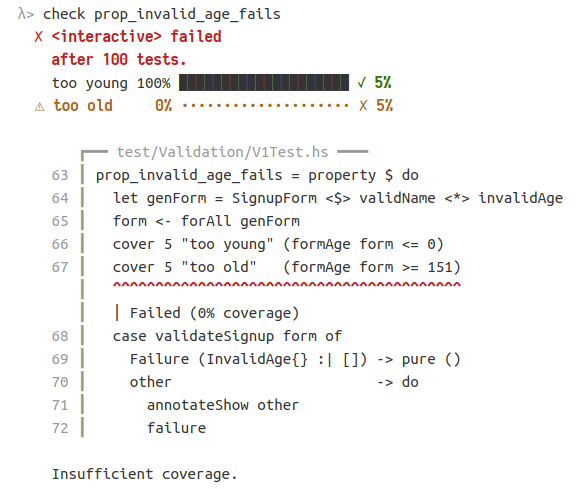
\includegraphics[width=.95\linewidth]{./pics/hedgehog1.png}
 \caption{Hedgehog fails}
 \label{fig:hedgehog1}
\end{figure}
\noindent 100\% too young and 0\% too old. The \texttt{invalidAge} generator is
clearly not good enough. Let's have a look at its definition again:

\begin{minted}{haskell}
invalidAge :: Gen Int
invalidAge = Gen.integral (Range.linear minBound 0)
\end{minted}
We're only generating invalid ages between the minimum bound of
\texttt{Int} and \texttt{0}. Let's fix that, by using
\texttt{Gen.choice} and another generator for ages greater than 150:

\begin{minted}{haskell}
invalidAge :: Gen Int
invalidAge = Gen.choice
  [ Gen.integral (Range.linear minBound 0)
  , Gen.integral (Range.linear 151 maxBound)
  ]
\end{minted}
Running tests again, the coverage check stops complaining. But there's
another problem:
\begin{figure}[htbp]
 \centering
 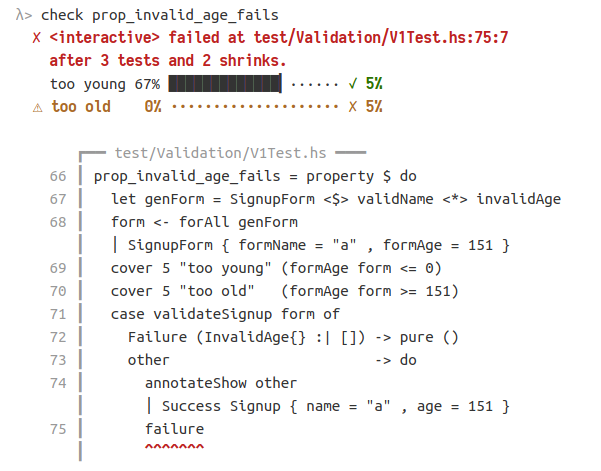
\includegraphics[width=.95\linewidth]{./pics/hedgehog2.png}
 \caption{Hedgehog fails}
 \label{fig:hedgehog2}
\end{figure}


\noindent OK, we have an actual bug. When the age is 151 or greater, the form is
deemed valid. It should cause a validation failure. Looking closer at
the implementation, we see that a pattern guard is missing the upper
bound check:

\begin{minted}{haskell}
validateAge age' | age' > 0  = Success (fromIntegral age')
                 | otherwise = Failure (pure (InvalidAge age'))
\end{minted}
If we change it to
\mintinline{haskell}{age' > 0 && age' <= 150},
and rerun the tests, they pass.

\begin{figure}[htbp]
 \centering
 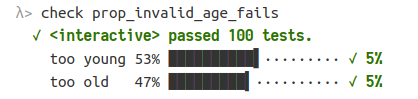
\includegraphics[width=.95\linewidth]{./pics/hedgehog3.png}
 \caption{Hedgehog passes}
 \label{fig:hedgehog3}
\end{figure}

\noindent We've fixed the bug.
Measuring and declaring requirements on coverage is a powerful tool in
Hedgehog. It gives us visibility into the generative tests we run,
making it practical to debug generators. It ensures our tests meet our
coverage requirements, even as implementation and tests evolve over
time.

\section{From Ages to Birth Dates}
\label{from-ages-to-birth-dates}

So far, our efforts have been successful. We've fixed real issues in
both implementation and tests. Management is pleased. They're now asking
us to modify the signup system, and use our testing skills to ensure
quality remains high.

Instead of entering their age, users will enter their birth date. Let's
suppose this information is needed for something important, like sending
out birthday gifts. The form validation function must be modified to
check, based on the supplied birth date date, if the user signing up is
old enough.

First, we import the \texttt{Calendar} module from the \texttt{time}
package:

\begin{minted}{haskell}
import           Data.Time.Calendar
\end{minted}
Next, we modify the \texttt{SignupForm} data type to carry a
\texttt{formBirthDate} of type \texttt{Date}, rather than an
\texttt{Int}.

\begin{minted}{haskell}
data SignupForm = SignupForm
  { formName      :: Text
  , formBirthDate :: Day
  } deriving (Eq, Show)
\end{minted}
And we make the corresponding change to the \texttt{Signup} data type:

\begin{minted}{haskell}
data Signup = Signup
  { name      :: Text
  , birthDate :: Day
  } deriving (Eq, Show)
\end{minted}
We've also been requested to improve the validation errors. Instead of
just \texttt{InvalidAge}, we define three constructors for various
invalid birthdates:

\begin{minted}{haskell}
data SignupError
  = NameTooShort Text
  | NameTooLong Text
  | TooYoung Day
  | TooOld Day
  | NotYetBorn Day
  deriving (Eq, Show)
\end{minted}
Finally, we need to modify the \texttt{validateSignup} function. Here,
we're faced with an important question. How should the validation
function obtain \emph{today's date}?

\subsection{Keeping Things
Deterministic}
\label{keeping-things-deterministic}

We could make \texttt{validateSignup} a non-deterministic action, which
in Haskell would have the following type signature:

\begin{minted}{haskell}
validateSignup
  :: SignupForm -> IO (Validation (NonEmpty SignupError) Signup)
\end{minted}
Note the use of \texttt{IO}. It means we could retrieve the current time
from the system clock, and extract the \texttt{Day} value representing
today's date. But this approach has severe drawbacks.

If \texttt{validateSignup} uses \texttt{IO} to retrieve the current
date, we can't test it with other dates. What it there's a bug that
causes validation to behave incorrectly only on a particular date? We'd
have to run the tests on that specific date to trigger it. If we
introduce a bug, we want to know about it \emph{immediately}. Not weeks,
months, or even years after the bug was introduced. Furthermore, if we
find such a bug with our tests, we can't easily reproduce it on another
date. We'd have to rewrite the implementation code to trigger the bug
again.

Instead of using \texttt{IO}, we'll use a simply technique for keeping
our function pure: take all the information the function needs as
arguments. In the case of \texttt{validateSignup}, we'll pass today's
date as the first argument:

\begin{minted}{haskell}
validateSignup
  :: Day -> SignupForm -> Validation (NonEmpty SignupError) Signup
\end{minted}
Again, let's not worry about the implementation just yet. We'll focus on
the tests.

\subsection{Generating Dates}
\label{generating-dates}

In order to test the new \texttt{validateSignup} implementation, we need
to generate \texttt{Day} values. We're going to use a few functions from
a separate module called \texttt{Data.Time.Gen}, previously written by
some brilliant developer in our team. Let's look at their type
signatures. The implementations are not very interesting.

The generator, \texttt{day}, generates a day within the given range:

\begin{minted}{haskell}
day :: Range Day -> Gen Day
\end{minted}
A day range is constructed with \texttt{linearDay}:

\begin{minted}{haskell}
linearDay :: Day -> Day -> Range Day
\end{minted}
Alternatively, we might use \texttt{exponentialDay}:

\begin{minted}{haskell}
exponentialDay :: Day -> Day -> Range Day
\end{minted}
The \texttt{linearDay} and \texttt{exponentialDay} range functions are
analoguous to Hedgehog's \texttt{linear} and \texttt{exponential} ranges
for integral numbers.

To use the generator functions from \texttt{Data.Time.Gen}, we first add
an import, qualified as \texttt{Time}:

\begin{minted}{haskell}
import qualified Data.Time.Gen      as Time
\end{minted}
Next, we define a generator \texttt{anyDay}:

\begin{minted}{haskell}
anyDay :: Gen Day
anyDay =
  let low  = fromGregorian 1900 1 1
      high = fromGregorian 2100 12 31
  in  Time.day (Time.linearDay low high)
\end{minted}
The date range [1900-01-01,2100-12-31]
is arbitrary. We could pick any centuries we like, provided the
\texttt{time} package supports the range. But why not make it somewhat
realistic?

\subsection{Rewriting Existing
Properties}
\label{rewriting-existing-properties}

Now, it's time to rewrite our existing property tests. Let's begin with
the one testing that validating a form with all valid data succeeds:

\begin{minted}{haskell}
prop_valid_signup_form_succeeds = property $ do
  today <- forAll anyDay                               -- (1)
  let genForm = SignupForm <$> validName <*> validBirthDate today
  form <- forAll genForm                               -- (2)

  case validateSignup today form of
    Success{}        -> pure ()
    Failure failure' -> do
      annotateShow failure'
      failure
\end{minted}
A few new things are going on here. We're generating a date representing
today (1), and generating a form with a birth date based on today's date
(2). Generating today's date, we're effectively time travelling and
running the form validation on that date. This means our
\texttt{validBirthDate} generator must know which date is today, in
order to pick a valid birth date. We pass today's date as a parameter,
and generate a date within the range of 18 to 150 years earlier:

\begin{minted}{haskell}
validBirthDate :: Day -> Gen Day
validBirthDate today = do
  n <- Gen.integral (Range.linear 18 150)
  pure (n `yearsBefore` today)
\end{minted}
We define the helper function \texttt{yearsBefore} in the test suite. It
offsets a date backwards in time by a given number of years:

\begin{minted}{haskell}
yearsBefore :: Integer -> Day -> Day
yearsBefore years = addGregorianYearsClip (negate years)
\end{minted}
The \texttt{Data.Time.Calendar} module exports the
\texttt{addGregorianYearsClip} function. It adds a number of years,
clipping February 29th (leap days) to February 28th where necessary.

Let's run tests:

\begin{quote}
$\lambda$\verb|> check prop_valid_signup_form_succeeds| \\
  \hspace*{1cm}\checkmark \verb|<interactive> passed 100 tests.|
\end{quote}
Let's move on to the next property, checking that invalid birth dates do
\emph{not} pass validation. Here, we use the same pattern as before,
generating today's date, but use \texttt{invalidBirthDate} instead:

\begin{minted}{haskell}
prop_invalid_age_fails = property $ do
  today <- forAll anyDay
  form <- forAll (SignupForm <$> validName <*> invalidBirthDate today)

  cover 5 "not yet born" (formBirthDate form > today)
  cover 5 "too young" (formBirthDate form > 18 `yearsBefore` today)
  cover 5 "too old" (formBirthDate form < 150 `yearsBefore` today)

  case validateSignup today form of
    Failure (TooYoung{}   :| []) -> pure ()
    Failure (NotYetBorn{} :| []) -> pure ()
    Failure (TooOld{}     :| []) -> pure ()
    other                        -> do
      annotateShow other
      failure
\end{minted}
Notice that we've also adjusted the coverage checks. There's a new
label, ``not born yet,'' for birth dates in the future. Running tests,
we see the label in action:

\begin{figure}[htbp]
 \centering
 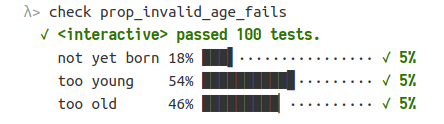
\includegraphics[width=.95\linewidth]{./pics/hedgehog4.png}
 \caption{Hedgehog results}
 \label{fig:hedgehog4}
\end{figure}

\noindent Good coverage, all tests passing. We're not quite done, though. There's
a particular set of dates that we should be sure to cover: ``today''
dates and birth dates that are close to, or exactly, 18 years apart.

Within our current property test for invalid ages, we're only sure that
generated birth dates include at least 5\% too old, and at least 5\% too
young. We don't know how far away from the ``18 years'' validation
boundary they are.

We could tweak our existing generators to produce values close to that
boundary. Given a date $T$, exactly 18 years before today's date, then:

\begin{itemize}

\item
  \texttt{invalidBirthDate} would need to produce birth dates just after
  but not equal to $T$  
\item
  \texttt{validBirthDate} would need to produce birth dates just before
  or equal to $T$
\end{itemize}
There's another option, though. Instead of defining separate properties
for valid and invalid ages, we'll use a \emph{single} property for all
cases. This way, we only need a single generator.

\section{A Single Validation
Property}
\label{a-single-validation-property}

In \href{https://www.youtube.com/watch?v=NcJOiQlzlXQ}{Building on
developers' intuitions to create effective property-based tests}, John
Hughes talks about ``one property to rule them all.'' Similarly, we'll
define a single property \texttt{prop\_validates\_age} for birth date
validation. We'll base our new property on
\texttt{prop\_invalid\_age\_fails}, but generalize to cover both
positive and negative tests:

\begin{minted}{haskell}
prop_validates_age = property $ do
  today <- forAll anyDay
  form  <- forAll (SignupForm <$> validName <*> anyBirthDate today) -- (1)

  let tooYoung        = formBirthDate form > 18 `yearsBefore` today -- (2)
      notYetBorn      = formBirthDate form > today
      tooOld          = formBirthDate form < 150 `yearsBefore` today
      oldEnough       = formBirthDate form <= 18 `yearsBefore` today
      exactly age = formBirthDate form == age `yearsBefore` today
      closeTo age =
        let diff' =
                diffDays (formBirthDate form) (age `yearsBefore` today)
        in  abs diff' `elem` [0 .. 2]

  cover 10 "too young"    tooYoung
  cover 1  "not yet born" notYetBorn
  cover 1  "too old"      tooOld

  cover 20 "old enough"   oldEnough                                 -- (3)
  cover 1  "exactly 18"   (exactly 18)
  cover 5  "close to 18"  (closeTo 18)

  case validateSignup today form of                                 -- (4)
    Failure (NotYetBorn{} :| []) | notYetBorn -> pure ()
    Failure (TooYoung{} :| []) | tooYoung -> pure ()
    Failure (TooOld{} :| []) | tooOld -> pure ()
    Success{} | oldEnough             -> pure ()
    other                             -> annotateShow other >> failure
\end{minted}
There are a few new things going on here:

\begin{enumerate}
\item
  Instead of generating exclusively invalid or valid birth dates, we're
  now generating \emph{any} birth date based on today's date
\item
  The boolean expressions are used both in coverage checks and in
  asserting, so we separate them in a \texttt{let} binding
\item
  We add three new labels for the valid cases
\item
  Finally, we assert on both valid and invalid cases, based on the same
  expressions used in coverage checks
\end{enumerate}
Note that our assertions are more specific than in
\texttt{prop\_invalid\_age\_fails}. The failure cases only pass if the
corresponding label expressions are true. The \texttt{oldEnough} case
covers all valid birth dates. Any result other than the four expected
cases is considered incorrect.

The \texttt{anyBirthDate} generator is based on today's date:

\begin{minted}{haskell}
anyBirthDate :: Day -> Gen Day
anyBirthDate today =
  let                                                      -- (1)
      inPast range = do   
        years <- Gen.integral range
        pure (years `yearsBefore` today)
      inFuture = do
        years <- Gen.integral (Range.linear 1 5)
        pure (addGregorianYearsRollOver years today)
      daysAroundEighteenthYearsAgo = do
        days <- Gen.integral (Range.linearFrom 0 (-2) 2)
        pure (addDays days (18 `yearsBefore` today))
  in                                                       -- (2)
      Gen.frequency
        [ (5, inPast (Range.exponential 1 150))
        , (1, inPast (Range.exponential 151 200))
        , (2, inFuture)
        , (2, daysAroundEighteenthYearsAgo)
        ]
\end{minted}
We defines helper functions (1) for generating dates in the past, in the
future, and close to 18 years ago. Using those helper functions, we
combine four generators, with different date ranges, using a
\texttt{Gen.frequency} distribution (1). The weights we use are selected
to give us a good coverage.
Let's run some tests (see figure \ref{fig:hedgehog5})
\begin{figure}[htbp]
 \centering
 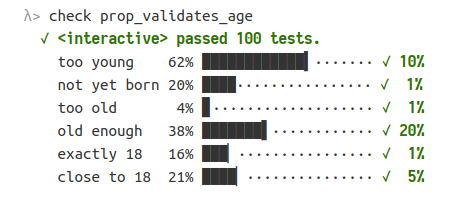
\includegraphics[width=.95\linewidth]{./pics/hedgehog5.png}
 \caption{Hedgehog results}
 \label{fig:hedgehog5}
\end{figure}

\noindent Looks good! We've gone from testing positive and negative cases
separately, to instead have a single property covering all cases, based
on a single generator. It's now easier to generate values close to the
valid/invalid boundary of our SUT, i.e.~around 18 years from today's
date.

\section{February 29th}
\label{february-29th}

For the fun of it, let's run some more tests. We'll crank it up to
20000 (see figure \ref{fig:hedgehog6}
\begin{figure}[htbp]
 \centering
 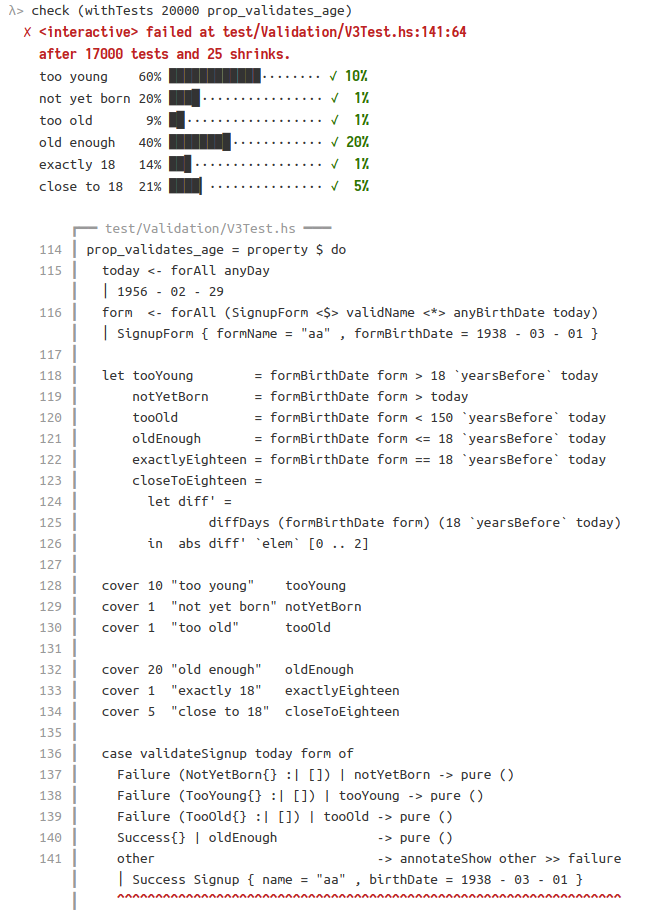
\includegraphics[width=\linewidth]{./pics/hedgehog6.png}
 \caption{Hedgehog results}
 \label{fig:hedgehog6}
\end{figure}

\noindent Failure! Chaos! What's going on here? Let's examine the test case:

\begin{itemize}

\item
  Today's date is 1956-02-29
\item
  The birth date is 1938-03-01
\item
  The validation function considers this \emph{valid} (it returns a
  \texttt{Success} value)
\item
  The test does considers this \emph{invalid} (\texttt{oldEnough} is
  \texttt{False})
\end{itemize}

This means that when the validation runs on a leap day,
\href{https://en.wikipedia.org/wiki/February_29\#Born_on_February_29}{February
29th}, and the person would turn 18 years old the day after (on March
1st), the validation function incorrectly considers the person old
enough. We've found a bug.

\subsection{Test Count and Coverage}
\label{test-count-and-coverage}

Two things led us to find this bug:

\begin{enumerate}
\item
  Most importantly, that we generate today's date and pass it as a
  parameter. Had we used the actual date, retrieved with an IO action,
  we'd only be able to find this bug every 1461 days. Pure functions are
  easier to test.
\item
  That we ran more tests than the default of 100. We might not have
  found this bug until much later, when the generated dates happened to
  trigger this particular bug. In fact, running 20000 tests does not
  always trigger the bug.
\end{enumerate}
Our systems are often too complex to be tested exhaustively. Let's use
our form validation as an example. Between 1900-01-01 and 2100-12-31
there are 73,413 days. Selecting today's date and the birth date from
that range, we have more than five billion combinations. Running that
many Hedgehog tests in GHCi on my laptop (based on some quick
benchmarks) would take about a month. And this is a simple pure
validation function!

To increase coverage, even if it's not going to be exhaustive, we can
increase the number of tests we run. But how many should we run? On a
continuous integration server we might be able to run more than we do
locally, but we still want to keep a tight feedback loop. And what if
our generators never produce inputs that reveal existing bugs,
regardless of the number of tests we run?

If we can't test exhaustively, we need to ensure our generators cover
interesting combinations of inputs. We need to carefully design and
measure our tests and generators, based on the edge cases we already
know of, as well as the ones that we discover over time. PBT without
measuring coverage easily turns into a false sense of security.

In the case of our leap day bug, we can catch it with fewer tests, and
on every test run. We need to make sure we cover leap days, used both as
today's date and as the birth date, even with a low number of tests.

\subsection{Covering Leap Days}
\label{covering-leap-days}

To generate inputs that cover certain edge cases, we combine specific
generators using \texttt{Gen.frequency}:

\begin{minted}{haskell}
(today, birthDate') <- forAll
  (Gen.frequency
    [ (5, anyDayAndBirthDate)                             -- (1)

    , (2, anyDayAndBirthDateAroundYearsAgo 18)            -- (2)
    , (2, anyDayAndBirthDateAroundYearsAgo 150)

    , (1, leapDayAndBirthDateAroundYearsAgo 18)           -- (3) 
    , (1, leapDayAndBirthDateAroundYearsAgo 150)

    , (1, commonDayAndLeaplingBirthDateAroundYearsAgo 18) -- (4)
    , (1, commonDayAndLeaplingBirthDateAroundYearsAgo 150)
    ]
  )
\end{minted}
Arbitrary values for today's date and the birth date are drawn most
frequently (1), with a weight of 5. Next, with weights of 2, are
generators for cases close to the boundaries of the validation function
(2). Finally, with weights of 1, are generators for special cases
involving leap days as today's date (3) and leap days as birth date (4).

Note that these generators return pairs of dates. For most of these
generators, there's a strong relation between today's date and the birth
date. For example, we can't first generate \emph{any} today's date, pass
that into a generator function, and expect it to always generate a leap
day that occured 18 years ago. Such a generator would have to first
generate the leap day and then today's date.

Let's define the generators. The first one, \texttt{anyDayAndBirthDate},
picks any today's date within a wide date range. It also picks a birth
date from an even wider date range, resulting in some future birth dates
and some ages above 150.

\begin{minted}{haskell}
anyDayAndBirthDate :: Gen (Day, Day)
anyDayAndBirthDate = do
  today <- Time.day
    (Time.linearDay (fromGregorian 1900 1 1)
                    (fromGregorian 2020 12 31)
    )
  birthDate' <- Time.day
    (Time.linearDay (fromGregorian 1850 1 1)
                    (fromGregorian 2050 12 31)
    )
  pure (today, birthDate')
\end{minted}
Writing automated tests with a hard-coded year 2020 might scare you.
Won't these tests fail when run in the future? No, not these tests.
Remember, the validation function is deterministic. We control today's
date. The \emph{actual} date on which we run these tests doesn't matter.

Similar to the previous generator is
\texttt{anyDayAndBirthDateAroundYearsAgo}. First, it generates any date
as today's date (1). Next, it generates an arbitrary date approximately
some number of years ago (2), where the number of years is an argument
of the generator.

\begin{minted}{haskell}
anyDayAndBirthDateAroundYearsAgo :: Integer -> Gen (Day, Day)
anyDayAndBirthDateAroundYearsAgo years = do
  today <- Time.day                                     -- (1)
    (Time.linearDay (fromGregorian 1900 1 1)
                    (fromGregorian 2020 12 31)
    )
  birthDate' <- addingApproxYears (negate years) today  -- (2)
  pure (today, birthDate')
\end{minted}
The \texttt{addingApproxYearsAgo} generator adds a number of years to a
date, and offsets it between two days back and two days forward in time.

\begin{minted}{haskell}
addingApproxYears :: Integer -> Day -> Gen Day
addingApproxYears years today = do
  days <- Gen.integral (Range.linearFrom 0 (-2) 2)
  pure (addDays days (addGregorianYearsRollOver years today))
\end{minted}
The last two generators used in our \texttt{frequency} distribution
cover leap day edge cases. First, let's define the
\texttt{leapDayAndBirthDateAroundYearsAgo} generator. It generates a
leap day used as today's date, and a birth date close to the given
number of years ago.

\begin{minted}{haskell}
leapDayAndBirthDateAroundYearsAgo :: Integer -> Gen (Day, Day)
leapDayAndBirthDateAroundYearsAgo years = do
  today      <- leapDay (Range.linear 1904 2020)
  birthDate' <- addingApproxYears (negate years) today
  pure (today, birthDate')
\end{minted}
The \texttt{leapDay} generator uses \texttt{mod} to only generate years
divisible by 4 and constructs dates on February 29th. That alone isn't
enough to only generate valid leap days, though. Years divisible by 100
but not by 400 are not leap years. To keep the generator simple, we
discard those years using the already existing \texttt{isLeapDay}
predicate as a filter.

\begin{minted}{haskell}
leapDay :: Range Integer -> Gen Day
leapDay yearRange = Gen.filter isLeapDay $ do
  year <- Gen.integral yearRange
  pure (fromGregorian (year - year `mod` 4) 2 29)
\end{minted}
In general, we should be careful about discarding generated values using
\texttt{filter}. If we discard too much, Hedgehog gives up and complains
loudly. In this particular case, discarding a few generated dates is
fine. Depending on the year range we pass it, we might not discard any
date.

Finally, we define the
\texttt{commonDayAndLeaplingBirthDateAroundYearsAgo} generator. It first
generates a leap day used as the birth date, and then a today's date
approximately the given number of years after the birth date.

\begin{minted}{haskell}
commonDayAndLeaplingBirthDateAroundYearsAgo :: Integer -> Gen (Day, Day)
commonDayAndLeaplingBirthDateAroundYearsAgo years = do
  birthDate' <- leapDay (Range.linear 1904 2020)
  today <- addingApproxYears years birthDate'
  pure (today, birthDate')
\end{minted}
That's it for the generators. Now, how do we know that we're covering
the edge cases well enough? With coverage checks!

\begin{minted}{haskell}

cover 5     -- (1)
      "close to 18, validated on common day"
      (closeTo 18 && not (isLeapDay today))
cover 1
      "close to 18, validated on leap day"
      (closeTo 18 && isLeapDay today)

cover 5     -- (2)
      "close to 150, validated on common day"
      (closeTo 150 && not (isLeapDay today))
cover 1
      "close to 150, validated on leap day"
      (closeTo 150 && isLeapDay today)

cover 5     -- (3)
      "exactly 18 today, born on common day"
      (exactly 18 && not (isLeapDay birthDate'))
cover       -- (4) 
  1
  "legally 18 today, born on leap day"
  (  isLeapDay birthDate'
  && (addGregorianYearsRollOver 18 birthDate' == today)
  )
\end{minted}
We add new checks to the property test, checking that we hit both leap
day and regular day cases around the 18th birthday (1) and the 150th
birthday (2). Notice that we had similar checks before, but we were not
discriminating between leap days and common days.

Finally, we check the coverage of two leap day scenarios that can occur
when a person
\href{https://en.wikipedia.org/wiki/February_29\#Legal_status}{legally
turns 18}: a person born on a common day turning 18 on a leap day (3),
and a leapling turning 18 on a common day (4).

Running the modified property test, we get the leap day counter-example
every time, even with as few as a hundred tests. For example, we might
see today's date being 1904-02-29 and the birth date being 1886-03-01.
The validation function deems the person old enough. Again, this is
incorrect.

Now that we can quickly and reliably reproduce the failing example we
are in a great position to find the error. While we could use a fixed
seed to reproduce the particular failing case from the 20000 tests run,
we are now more confident that the property test would catch future leap
day-related bugs, if we were to introduce new ones. Digging into the
implementation, we'll find a boolean expression in a pattern guard being
the culprit:

\begin{minted}{haskell}
birthDate' <= addGregorianYearsRollOver (-18) today
\end{minted}
The use of \texttt{addGregorianYearsRollOver} together with adding a
negative number of years is the problem, rolling over to March 1st
instead of clipping to February 28th. Instead, we should use
\texttt{addGregorianYearsClip}:

\begin{minted}{haskell}
birthDate' <= addGregorianYearsClip (-18) today
\end{minted}
Running 100 tests again, we see that they all pass, and that our
coverage requirements are met.

\begin{figure}[htbp]
 \centering
 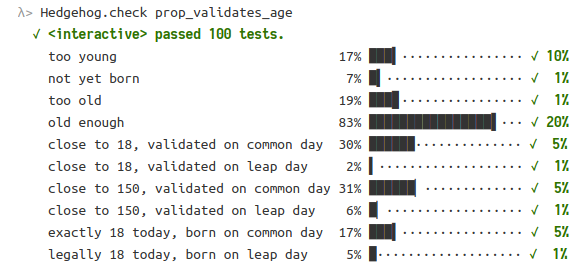
\includegraphics[width=\linewidth]{./pics/hedgehog7.png}
 \caption{Hedgehog results}
 \label{fig:hedgehog7}
\end{figure}

\section{Summary}
\label{summary}

In this tutorial, we started with a simple form validation function,
checking the name and age of a person signing up for an online service.
We defined property tests for positive and negative tests, learned how
to test generators with coverage checks, and found bugs in both the test
suite and the implementation.

When requirements changed, we had to start working with dates. In order
to keep the validation function deterministic, we had to pass in today's
date. This enabled us to simulate the validation running on any date, in
combination with any reported birth date, and trigger bugs that could
otherwise take years to find, if ever. Had we not made it deterministic,
we would likely not have found the leap day bug later on.

To generate inputs that sufficiently test the validation function's
boundaries, we rewrote our separate positive and negative properties
into a single property, and used coverage checks to ensure the quality
of our generators. The trade-off between multiple disjoint properties
and a single more complicated property is hard.

With multiple properties, for example split between positive and
negative tests, both generators and assertions can be simpler and more
targeted. On the other hand, you run a risk of missing certain inputs.
The set of properties might not cover the entire space of inputs.
Furthermore, performing coverage checks across multiple properties,
using multiple targeted generators, can be problematic.

Ensuring coverage of generators in a single property is easier. You
might even get away with a naive generator, depending on the system
you're testing. If not, you'll need to combine more targeted generators,
for example with weighted probabilities. The drawback of using a single
property is that the assertion not only becomes more complicated, it's
also likely to mirror the implementation of the SUT. As we saw with our
single property testing the validation function, the assertion
duplicated the validation rules. You might be able to reuse the coverage
expressions in assertions, but still, there's a strong coupling.

The choice between single or multiple properties comes down to
\emph{how} you want to cover the boundaries of the SUT. Ultimately, both
approaches can achieve the same coverage, in different ways. They both
suffer from the classic problem of a test suite mirroring the system
it's testing.

Finally, running a larger number of tests, we found a bug related to
leap days. Again, without having made the validation function
deterministic, this could've only been found on a leap day. We further
refined our generators to cover leap day cases, and found the bug
reliably with as few as 100 tests. The bug was easy to find and fix when
we had the inputs pointing directly towards it.

That's it for this tutorial. Thanks for reading, and happy property
testing and time travelling!
